%appendices
\begin{appendices}
\section{Figures}
\label{appendix:countfigs}

\begin{figure}[H]
	\centering
	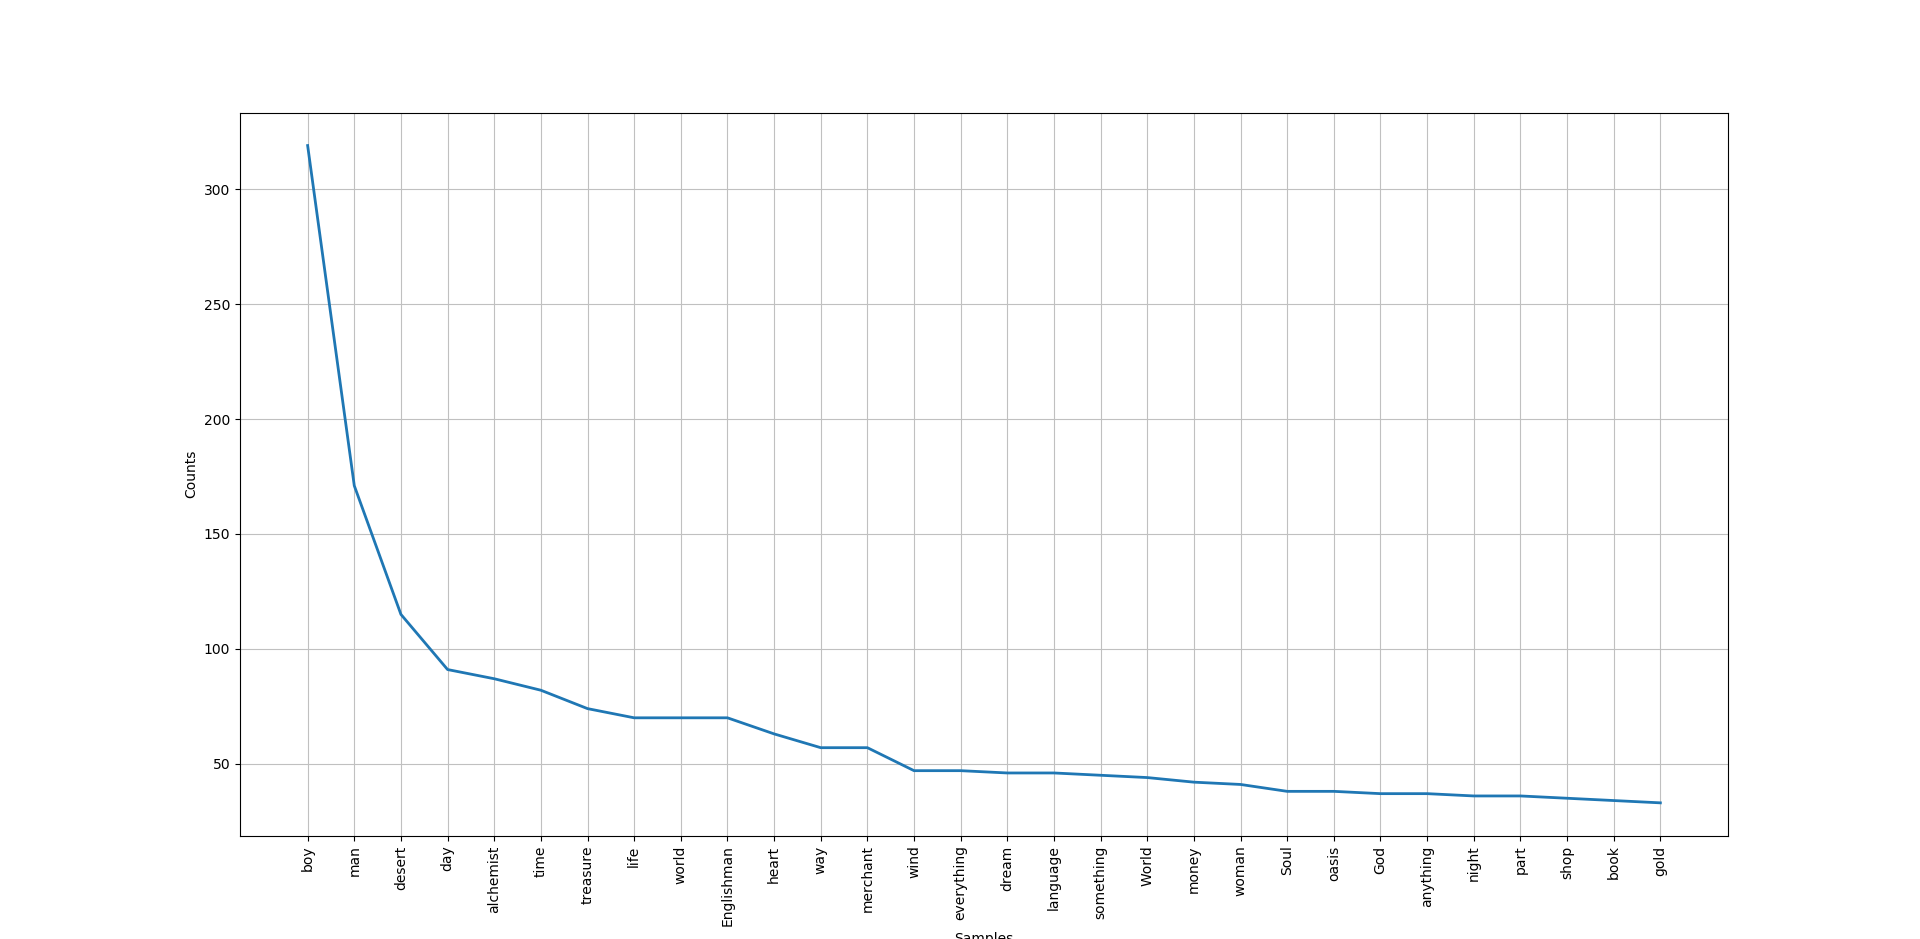
\includegraphics[width=1\linewidth]{the_alchemist_nouns}
	\caption{Most used nouns in The Alchemist}\label{fig:the_alchemist_nouns}
\end{figure}

\begin{figure}[H]
	\centering
	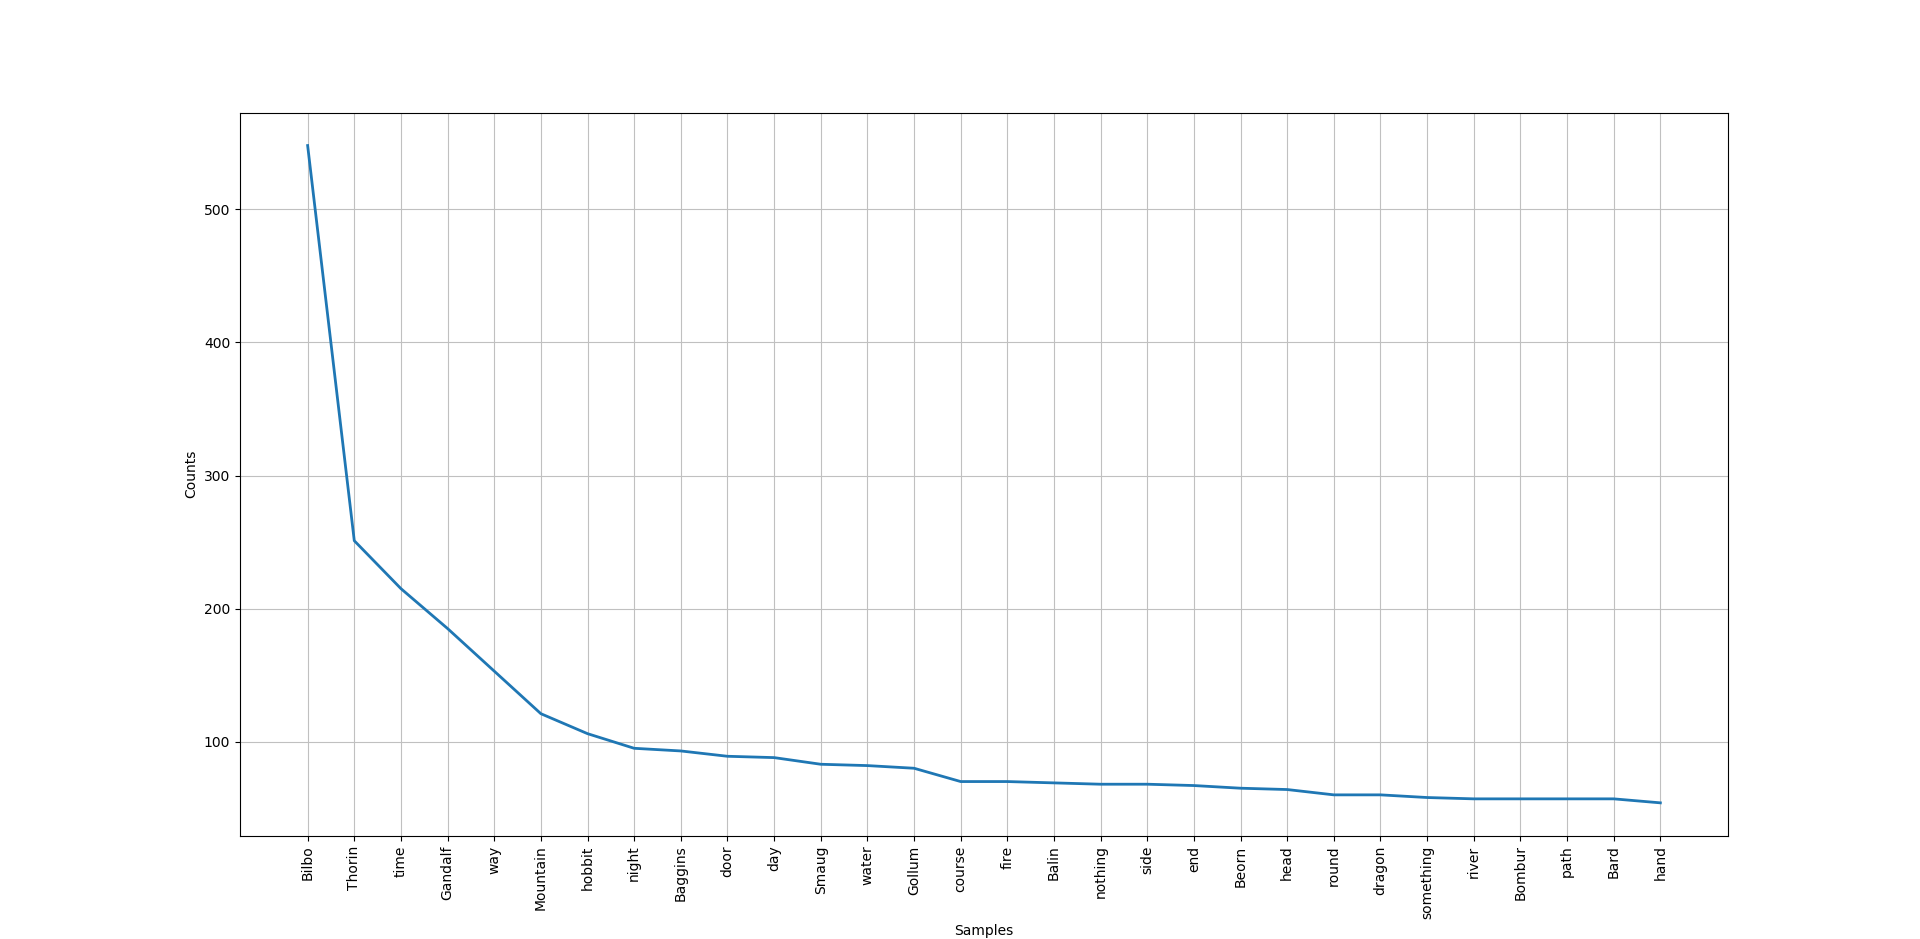
\includegraphics[width=1\linewidth]{the_hobbit_nouns}
	\caption{Most used nouns in The Hobbit}\label{fig:the_hobbit_nouns}
\end{figure}

\begin{figure}[H]
	\centering
	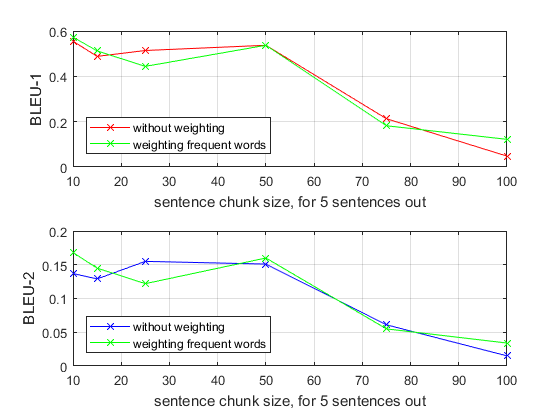
\includegraphics[width=0.7\linewidth]{bleus_okay}
	\caption{BLEU scores for varying the section size with constant 5 sentences out per step for the Alchemist. }\label{fig:bleus_okay}
\end{figure}


\section{Individual contributions}
As planned at the start, the tasks were split fairly evenly. All have worked on the report consistently, with Jonas and Taesoo focusing more on the programming, and Sangitha on dataset collection and experiment evaluation.

\end{appendices}